\documentclass{ieeeaccess}
\usepackage{cite}
\usepackage{amsmath,amssymb,amsfonts}
\usepackage{algorithmic}
\usepackage{graphicx}
\usepackage{textcomp}
\usepackage{booktabs}
\usepackage{array}

\usepackage{bm}
\makeatletter
\AtBeginDocument{\DeclareMathVersion{bold}
\SetSymbolFont{operators}{bold}{T1}{times}{b}{n}
\SetSymbolFont{NewLetters}{bold}{T1}{times}{b}{it}
\SetMathAlphabet{\mathrm}{bold}{T1}{times}{b}{n}
\SetMathAlphabet{\mathit}{bold}{T1}{times}{b}{it}
\SetMathAlphabet{\mathbf}{bold}{T1}{times}{b}{n}
\SetMathAlphabet{\mathtt}{bold}{OT1}{pcr}{b}{n}
\SetSymbolFont{symbols}{bold}{OMS}{cmsy}{b}{n}
\renewcommand\boldmath{\@nomath\boldmath\mathversion{bold}}}
\makeatother

\def\BibTeX{{\rm B\kern-.05em{\sc i\kern-.025em b}\kern-.08em
    T\kern-.1667em\lower.7ex\hbox{E}\kern-.125emX}}

% ---- paper-specific shortcuts ----
\newcommand{\Ghat}{\hat{G}}
\newcommand{\amin}{\alpha_{\min}}
\newcommand{\amax}{\alpha_{\max}}
\newcommand{\Estable}{E_{\mathrm{stable}}}
\newcommand{\Edelta}{E_{\Delta}}
\newcommand{\pmsd}[2]{#1{\scriptstyle\pm #2}}

% ---- biography spacing (ieeeaccess.cls left untouched) ----
% Same as the class's IEEEbiographynophoto, except the gap before each
% biography is 1.5 baselines (class default: 4 baselines).
\makeatletter
\renewenvironment{IEEEbiographynophoto}[1]{%
\addcontentsline{toc}{subsection}{#1}%
\normalfont\biographyfont\interlinepenalty500%
\vskip 1.5\baselineskip plus 1fil minus 0\baselineskip%
\parskip=0pt\par%
\noindent{\biographyheadfont\uppercase{#1}\ }\@IEEEgobbleleadPARNLSP}{\relax\par\normalfont}
\makeatother

%Your document starts from here ___________________________________________________
\begin{document}

\title{Selective Causal Adaptation for Evolving Time-Series Graphs: A Stability--Plasticity Study}
\author{\uppercase{Suyesha Saha}\authorrefmark{1},
\uppercase{Ippili Sai Sahasra}\authorrefmark{1},
\uppercase{Ananya Arumbakkam}\authorrefmark{1}, AND
\uppercase{Suhasini S}\authorrefmark{2}}

\address[1]{School of Computer Science and Engineering, Vellore Institute of Technology, Chennai, India (e-mail: suyesha.saha2024@vitstudent.ac.in, ippili.saisahasra2024@vitstudent.ac.in, ananya.arumbakkam2024@vitstudent.ac.in)}
\address[2]{School of Electronics Engineering, Vellore Institute of Technology, Chennai, India (e-mail: suhasini.s@vit.ac.in)}

\markboth
{Saha \headeretal: Selective Causal Adaptation for Evolving Time-Series Graphs}
{Saha \headeretal: Selective Causal Adaptation for Evolving Time-Series Graphs}

\corresp{Corresponding author: Suhasini S (e-mail: suhasini.s@vit.ac.in).}

\begin{abstract}
Selective Causal Adaptation (SCA) is a training-free streaming estimator for evolving, lagged predictive graphs. It combines a local past-only regression estimate with graph memory, a two-window change signal, and edge-specific persistence and deviation signals. These components determine an edgewise plasticity rate for updating the remembered graph. SCA is evaluated on recurring-regime synthetic data, a development ablation, and an illustrative Causal Chambers series. A held-out high-dimensional stress test ($d=50$, $L=4$, Gaussian measurement noise $\sigma=0.10$) shows that a dimension-aware ridge configuration ($W=1000$, $D=500$, ridge alpha $=1.0$) repairs a documented small-window OLS failure: it obtains F1 $0.576\pm0.036$, AUPRC $0.831\pm0.014$, and an eligible-update null false-alarm rate of $0.044\pm0.014$ over seeds 20--39. This targeted result does not establish broad superiority over rolling or regime-aware alternatives. We therefore present SCA as a past-only Granger-style predictive graph estimator, document the remaining limitations of its evaluation, and distinguish completed evidence from pending matched-baseline and full-factorial studies.
\end{abstract}

\begin{keywords}
Granger-style predictive graphs, streaming estimation, edge-level plasticity, non-stationary time series, regime-change detection, stability--plasticity trade-off, structural Hamming distance.
\end{keywords}

\titlepgskip=-21pt

\maketitle

%=====================================================================
\section{Introduction}
\label{sec:introduction}
\PARstart{M}{ultivariate} time series may exhibit non-stationary predictive relationships, motivating methods that estimate lagged graphs while preserving temporal order \cite{r1,r5}. This paper considers piecewise-stationary synthetic processes in which a small subset of lagged relationships changes at known evaluation boundaries while other relationships remain unchanged.

Classical time-series causal-discovery methods such as PCMCI+ and DYNOTEARS are commonly evaluated under a stationary generating mechanism. A second family addresses non-stationarity through regime discovery, including CD-NOD, RPCMCI, CASTOR, and FANTOM. These approaches estimate structures at the regime or graph level. Edge-level memory may be useful when only a subset of lagged relationships changes; this is the restricted setting examined here.

This paper studies edgewise adaptation of a lagged predictive graph. SCA is a streaming, training-free estimator that maintains graph memory and updates each candidate lagged edge with its own plasticity rate. The rate is high only when a graph-level change signal, local disagreement, and persistent disagreement coincide. Otherwise, the rate remains near a small floor.

SCA is deliberately implemented on top of a transparent, regression-based, past-only (Granger-style) evidence score rather than a trained neural encoder. This keeps the pipeline free of gradient-based training, makes every design decision traceable to a closed-form update rule, and keeps the computational footprint small enough for streaming or embedded causal monitoring.

The paper asks three restricted questions. \textbf{RQ1:} How does persistence-gated memory behave relative to a memory-free rolling estimator on the reported synthetic settings? \textbf{RQ2:} What qualitative effect do persistence and edgewise gating have in the development ablation? \textbf{RQ3:} What does the completed d=50, L=4 stress test reveal about the role of regression conditioning and detector calibration?

We report a controlled recurring-regime synthetic benchmark, a four-variable development ablation, an illustrative Causal Chambers evaluation, and a completed held-out d=50, L=4 stress-test repair. The legacy fixed-configuration factorial tables are retained only as diagnostics, not as primary evidence. Matched held-out KGLS, RLS, global-rate EMA, locality-sweep, and broad jointly tuned factorial results are not yet available.

\noindent\textit{Contributions.} This paper contributes: (1) a graph-memory framework for evolving lagged predictive graphs that separates a local, past-only evidence estimator from persistent memory; (2) a persistence-gated, edgewise plasticity mechanism; (3) a documented legacy factorial diagnostic and a jointly tuned, null-calibrated d=50, L=4 held-out stress-test repair; and (4) an explicit account of the method's empirical scope and limitations. The paper does not claim universal superiority or structural-causal identification.

%=====================================================================
\section{Related Work}
\label{sec:related}
Causal discovery from stationary time series is a mature area. PCMCI and its extension PCMCI+ \cite{r1} combine a condition-selection stage with conditional-independence testing to recover lagged and (in PCMCI+) contemporaneous links, scaling to moderately high dimensions but assuming a single stationary regime. DYNOTEARS \cite{r2,r3} casts structure learning as continuous, acyclicity-constrained optimisation over both instantaneous and lagged adjacency matrices, building on the NOTEARS acyclicity characterisation. Rhino \cite{r4} relaxes the constant-variance assumption to history-dependent noise but still fits a single graph to the whole series. All three approaches degrade once the generating mechanism itself changes over time, motivating the regime-aware literature discussed next.

A second line of work targets non-stationarity directly by discovering regimes. CD-NOD \cite{r5} treats the time index as a surrogate variable, detects change points through the variability of conditional distributions, and returns a single summary graph whose parents are the union of per-regime parents. RPCMCI \cite{r6} learns a temporal graph per regime. CASTOR \cite{r7}, FANTOM \cite{r8}, and SPACETIME \cite{r9} represent further regime-aware approaches. Temporal graph attention networks \cite{r10} target dynamic link prediction rather than the lagged predictive-graph estimation considered here.

The common feature of CD-NOD, RPCMCI, CASTOR, and FANTOM is that adaptation is formulated at the level of the whole graph (or, for CD-NOD, a single summary graph): a regime boundary triggers estimation of a new structure. This is well matched to settings where a regime shift touches most of the mechanism, and FANTOM in particular provides identifiability guarantees that the present, purely empirical study does not attempt to match. SCA instead targets the complementary setting of localised non-stationarity, in which only a subset of edges is perturbed at a change point, by moving the unit of adaptation to the individual edge and combining a lightweight two-window change detector with an edge-specific persistence tracker. This design trades the richer generative assumptions and identifiability results of FANTOM-style models for a training-free, closed-form update rule with a small, fixed memory footprint.

Benchmarking resources for this literature include the TimeGraph synthetic suite \cite{r11}, the physical Causal Chambers wind-tunnel testbed \cite{r12}, and EEG seizure corpora documented to exhibit heteroscedastic sensor noise \cite{r8,r13}; we draw on the Causal Chambers wind-tunnel data for the external benchmark reported in Section~\ref{res:chambers}. Identifiability of additive-noise causal models under the causal Markov, minimality, sufficiency, and (within-regime) stationarity assumptions is established in \cite{r14} and extended to heteroscedastic and multi-regime settings in \cite{r8}; SCA relies on this line of results only informally, as a justification for using a regression-based evidence score as a proxy for edge presence, rather than proving a new identifiability result of its own.

%=====================================================================
\section{Problem Formulation}
\label{sec:problem}
Let $X=\{x_t\}_{t=1}^{T}$ denote a $d$-dimensional multivariate time series, $x_t\in\mathbb{R}^{d}$. A time-varying causal graph is represented by a tensor $G_t\in\mathbb{R}^{d\times d\times(L+1)}$, where the third index is the lag $\ell\in\{0,1,\dots,L\}$. We assume a piecewise-constant generating graph with unknown regime-change points $\tau$, so that between consecutive change points the graph is fixed and equal to some regime graph (denoted $A$ for the regime immediately before a transition and $B$ for the regime immediately after). We define the \textbf{stable edge set} and the \textbf{changed edge set} at a transition as
\begin{align}
\Estable &= B\cap A, \label{eq:stable}\\
\Edelta &= (B\setminus A)\cup(A\setminus B), \label{eq:changed}
\end{align}
so that $\Edelta$ collects every edge that is added or removed by the transition, and $\Estable$ collects every edge whose lagged coefficient is unchanged. The estimation problem is to produce, at every time step $t$, an estimate that jointly satisfies two objectives:

\textbf{Stability:} for $(i,j,\ell)\in\Estable$, the estimate at time $t$ should continue to match its pre-transition value once the transition has occurred, i.e., the memory should not be disturbed by a change elsewhere in the graph.

\textbf{Plasticity:} for $(i,j,\ell)\in\Edelta$, the estimate should converge to its post-transition value as quickly as possible once the transition has occurred.

These two objectives are in direct tension: a memory mechanism aggressive enough to track $\Edelta$ quickly will, absent an edge-specific gating signal, also perturb $\Estable$, while a memory mechanism conservative enough to fully protect $\Estable$ will adapt $\Edelta$ slowly. Section~\ref{sec:sca} formalises SCA as a mechanism that resolves this tension at the level of the individual edge $(i,j,\ell)$ rather than through a single global learning rate. We also note explicitly, consistent with the discussion in Section~\ref{sec:limits}, that the estimator considered here is a past-only (Granger-style) predictive estimator: it regresses each target on lagged predictors only, the lag-0 (contemporaneous) plane is fixed to zero throughout, and no claim is made that the identified relationships correspond to contemporaneous structural causal effects in the sense of Pearl's do-calculus.

%=====================================================================
\section{Selective Causal Adaptation}
\label{sec:sca}
SCA processes the series causally: only samples up to and including the current time step are used at every stage. The pipeline (Fig.~\ref{fig:arch}) has six components run once per time step over a trailing window of length $W$: a local graph estimator, a two-window change detector, an edge-level deviation and persistence tracker, a plasticity gate, and a memory update. Fig.~\ref{fig:plasticity} illustrates how the resulting plasticity rate separates the fate of a stable edge from that of a changed edge.

\begin{figure}[!t]
\centering
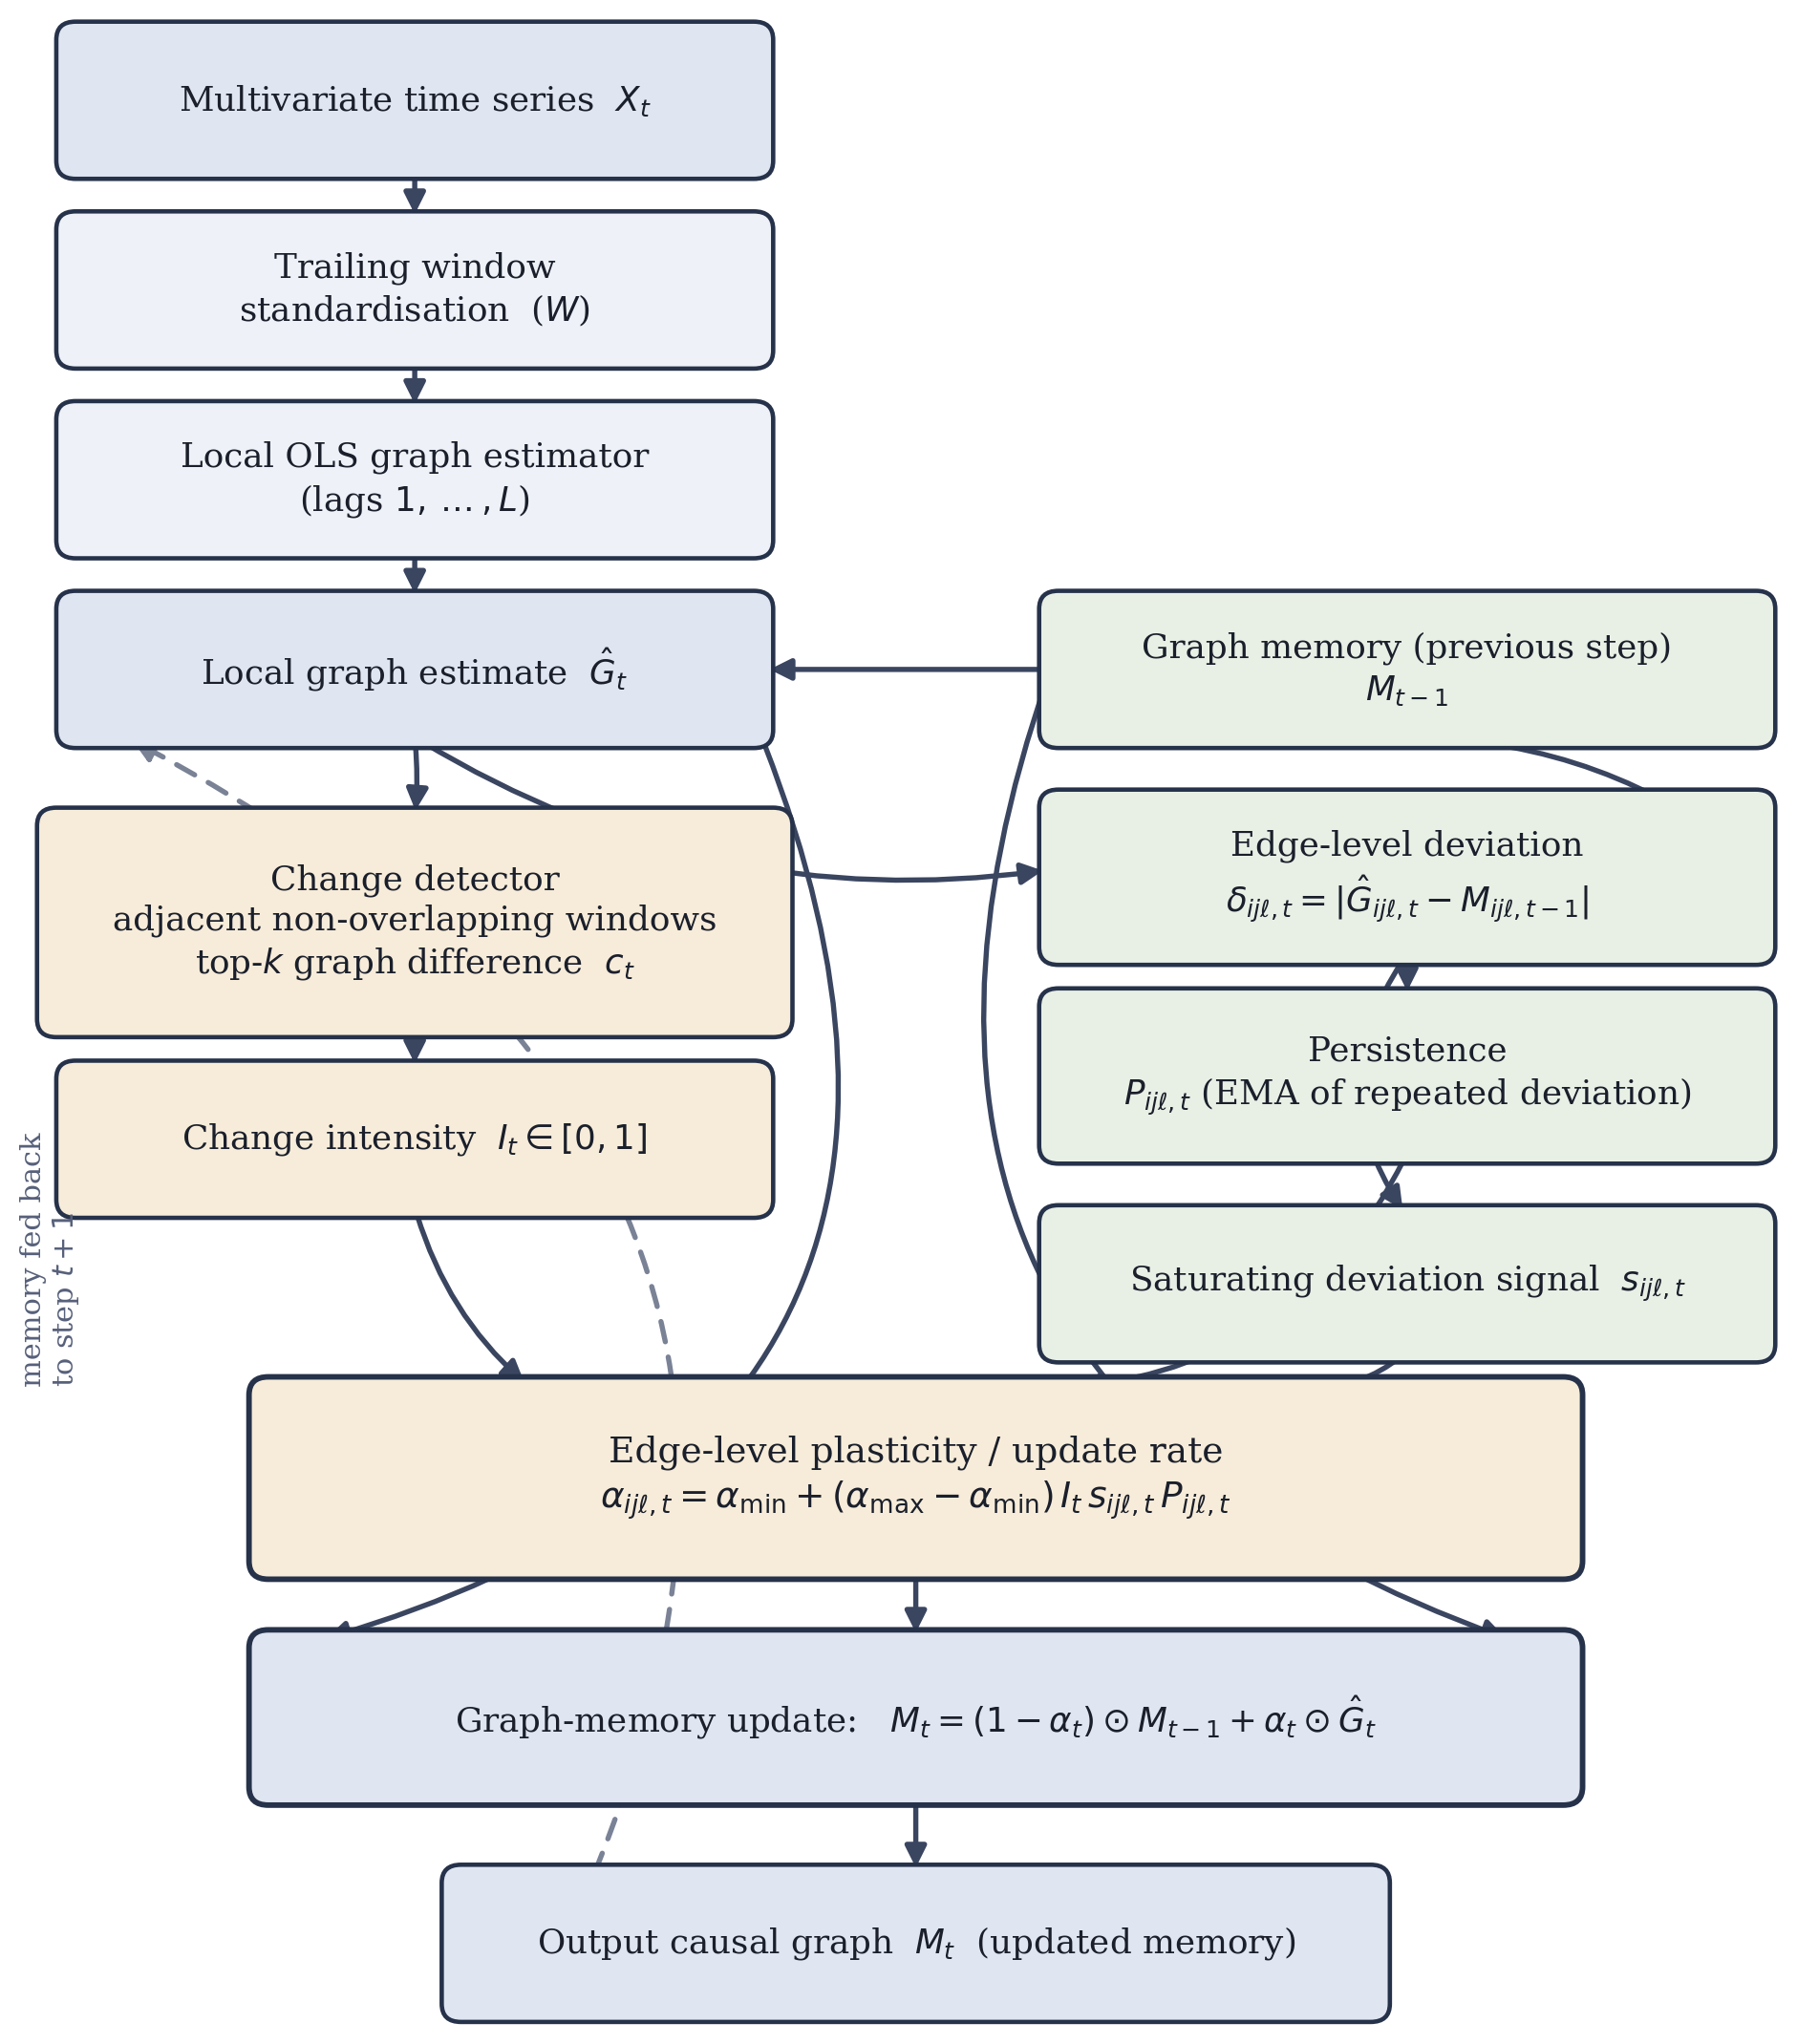
\includegraphics[width=0.98\columnwidth]{figs/image1.png}
\caption{\textbf{Overall SCA architecture.} A local OLS graph estimate is compared against graph memory; a two-window change detector and an edge-level deviation/persistence pathway jointly gate a per-edge plasticity rate that updates the memory at every step.}
\label{fig:arch}
\end{figure}

\begin{figure}[!t]
\centering
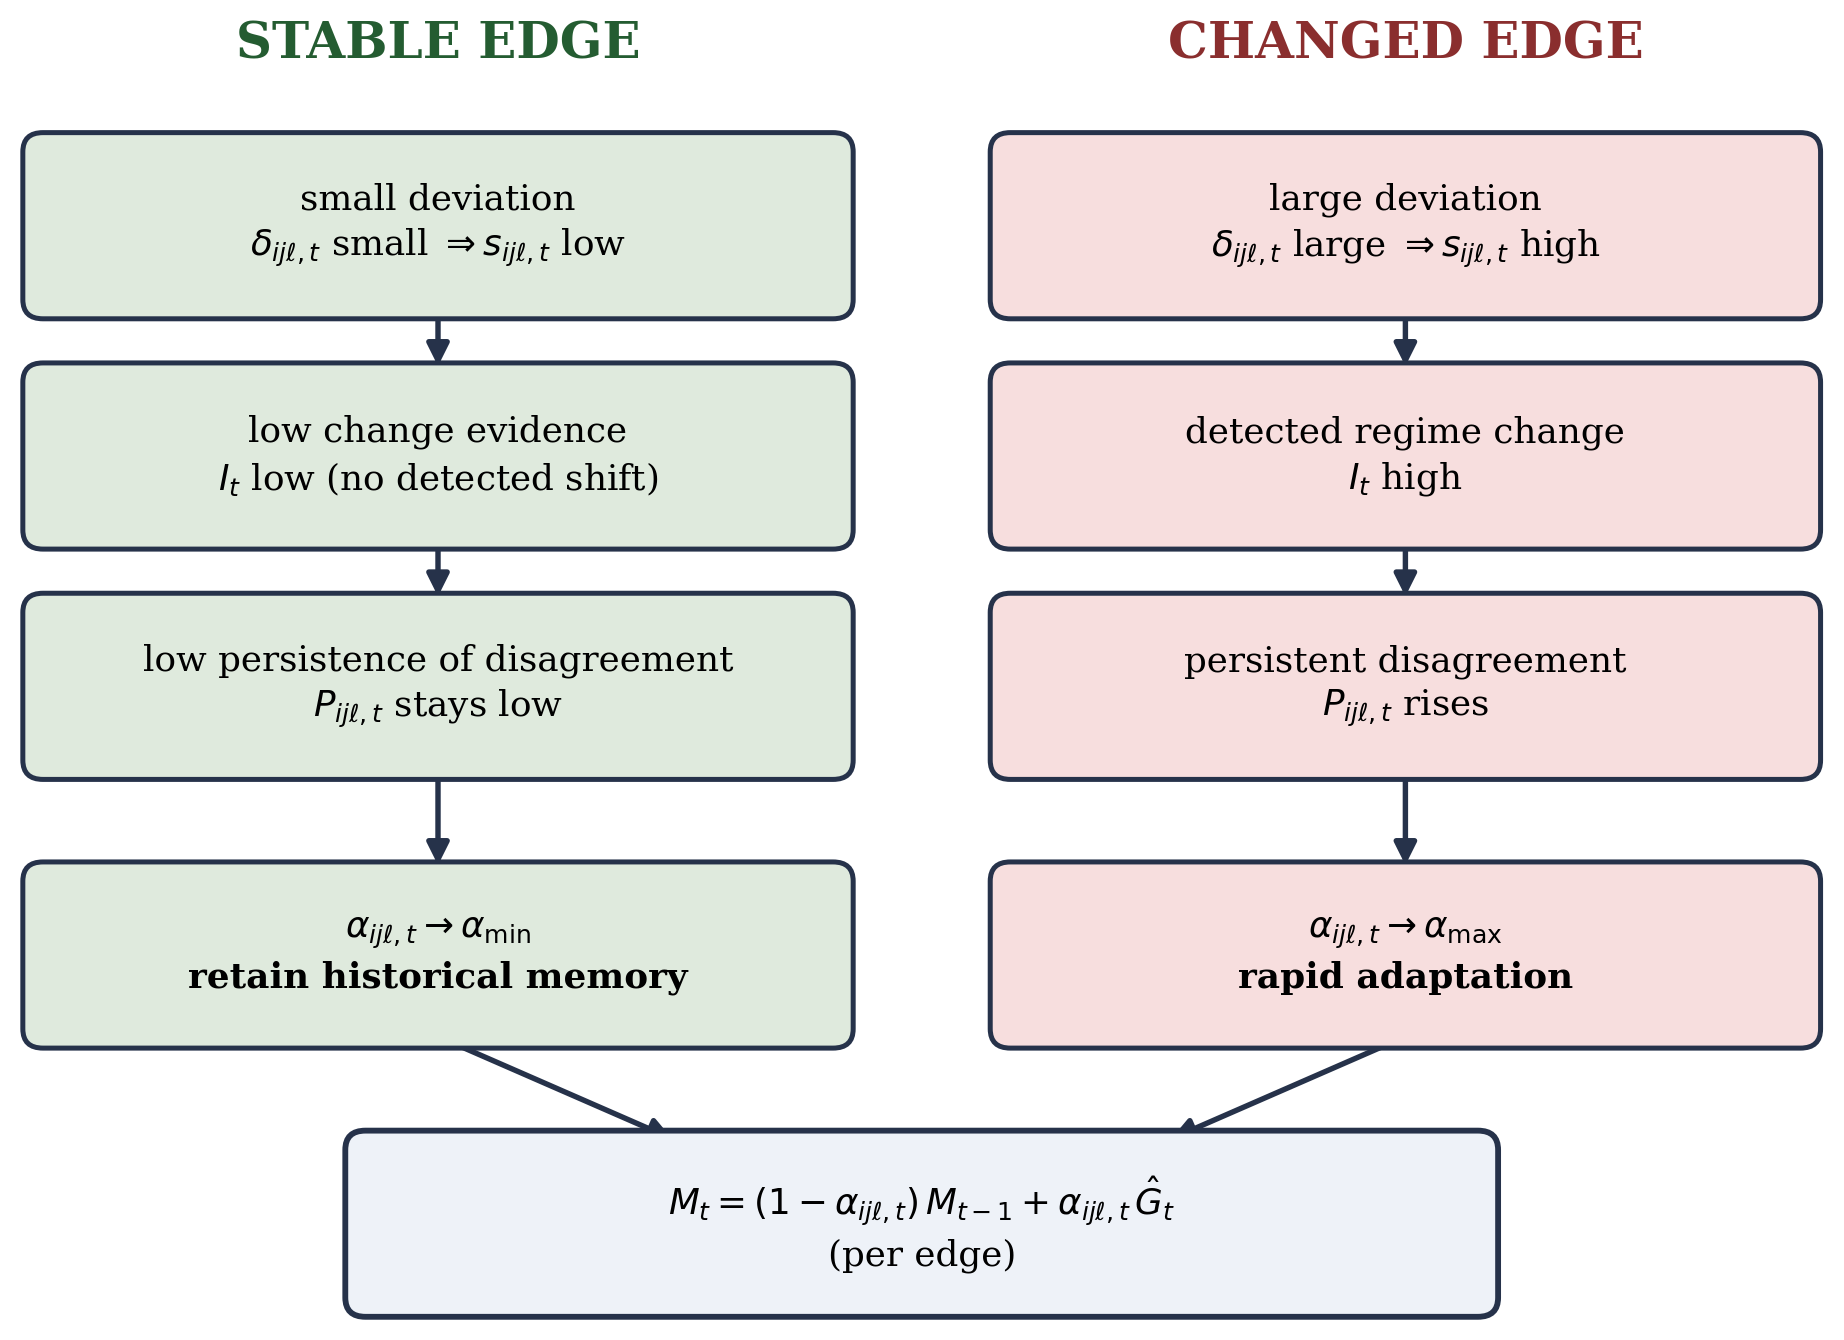
\includegraphics[width=0.98\columnwidth]{figs/image2.png}
\caption{\textbf{Stability--plasticity mechanism.} A stable edge accumulates low deviation, change intensity, and persistence, so its plasticity collapses toward $\amin$; a changed edge accumulates high values of all three and its plasticity approaches $\amax$.}
\label{fig:plasticity}
\end{figure}

\subsection{Local Graph Estimation}
\label{sec:local}
Within a trailing window, the variables are standardised and a joint multivariate least-squares (OLS) model is fit:
\begin{equation}
x'_t=\beta_0+\sum_{\ell=1}^{L}B_\ell\,x'_{t-\ell},
\label{eq:ols}
\end{equation}
and the local graph estimate is read off as the regression coefficients,
\begin{equation}
\Ghat_{ij\ell,t}=[B_\ell]_{ij}
\label{eq:ghat}
\end{equation}
for lags $\ell=1,\dots,L$. The lag-zero plane is fixed to zero throughout, since conditioning on $X_i(t)$ to predict $X_j(t)$ is not identifiable from observational data without further structural assumptions and would additionally introduce contemporaneous-leakage artefacts in a streaming setting; diagonal (self-loop) entries are likewise removed. Consequently $\Ghat$ is a past-only, Granger-style estimator: it reflects predictive, lagged dependence, not necessarily an instantaneous structural mechanism.

\subsection{Change Detection}
\label{sec:detect}
To decide whether the series is currently undergoing a genuine, graph-wide structural change, two adjacent, non-overlapping windows of length $D$ immediately preceding $t$ are each summarised into a local graph, and the $k$ largest entries of their absolute difference (after zeroing the diagonal) are averaged into a scalar change score:
\begin{equation}
c_t=\operatorname{mean}\bigl(\operatorname{top}_k\bigl(\lvert\Ghat_{\mathrm{rec},t}-\Ghat_{\mathrm{prev},t}\rvert\bigr)\bigr)
\label{eq:score}
\end{equation}
with $k=\min\bigl(4,\,d^2(L+1)\bigr)$. Using only the strongest few edge deviations, rather than an average over the entire graph, keeps the statistic sensitive to a small number of genuinely perturbed edges without being diluted by the $d^2(L+1)$ entries that typically remain unchanged. The corresponding global change intensity is
\begin{equation}
I_t=\begin{cases}\min(1,\,c_t/\theta) & \text{if } c_t\ge\theta,\\[2pt] 0 & \text{otherwise,}\end{cases}
\label{eq:intensity}
\end{equation}
where $\theta$ controls detector sensitivity and $I_t\in[0,1]$ represents the strength of any detected structural change. $I_t=0$ whenever no change is flagged, so that no edge receives a boosted plasticity rate in the absence of a detected shift.

\subsection{Edge-Level Deviation and Persistence}
\label{sec:edge}
For every candidate edge $(i,j,\ell)$, the deviation between the freshly estimated local graph and the current memory is
\begin{equation}
\delta_{ij\ell,t}=\lvert\Ghat_{ij\ell,t}-M_{ij\ell,t-1}\rvert.
\label{eq:dev}
\end{equation}
Persistence captures repeated evidence that an edge differs from its remembered value, via an exponential moving average of an indicator that the deviation exceeds a small tolerance $\epsilon$:
\begin{equation}
P_{ij\ell,t}=\lambda P_{ij\ell,t-1}+(1-\lambda)\,\mathbb{1}\bigl[\delta_{ij\ell,t}\ge\epsilon\bigr],
\label{eq:persist}
\end{equation}
so a single noisy window cannot, by itself, push an edge's persistence score to a high value; $P$ rises only when the disagreement between the local estimate and memory is sustained across several consecutive steps. Finally, the raw deviation is mapped to a bounded, saturating signal,
\begin{equation}
s_{ij\ell,t}=\frac{\delta_{ij\ell,t}}{\delta_{ij\ell,t}+\epsilon}\in[0,1),
\label{eq:sat}
\end{equation}
which grows quickly for small deviations and saturates for large ones, preventing an occasional very large outlier from dominating the plasticity rate.

\subsection{Plasticity Update}
\label{sec:plastic}
The three signals above---whether the graph as a whole is changing ($I_t$), whether this particular edge is currently deviating from memory ($s_{ij\ell,t}$), and whether that deviation has persisted ($P_{ij\ell,t}$)---are combined multiplicatively into a single edge-level plasticity (update) rate, mapped into an admissible range $[\amin,\amax]$:
\begin{equation}
\alpha_{ij\ell,t}=\amin+(\amax-\amin)\,I_t\,s_{ij\ell,t}\,P_{ij\ell,t},
\label{eq:alpha}
\end{equation}
with diagonal entries then set to zero. This multiplicative structure is central to the mechanism: aggressive updating of an edge occurs only when (1) a structural change has been detected somewhere in the graph, (2) the local estimate disagrees with graph memory for this specific edge, and (3) that disagreement has persisted across recent steps. If any one of the three factors is near zero, the product collapses toward $\amin$ and the edge's memory entry is barely disturbed, which is precisely the mechanism that protects an unrelated stable edge from a regime change occurring elsewhere in the graph. Conversely, $\amin>0$ is set strictly positive so that even edges not flagged by the detector retain a small, non-zero rate of slow adaptation (drift), rather than being frozen indefinitely.

\subsection{Graph-Memory Update}
\label{sec:memory}
The memory tensor is updated using a per-edge exponential moving average, controlled by the edge-level plasticity rate:
\begin{equation}
M_t=(1-\alpha_t)\odot M_{t-1}+\alpha_t\odot\Ghat_t,
\label{eq:memory}
\end{equation}
where $\odot$ denotes element-wise multiplication and the memory tensor $M_t$ is emitted directly as the model's causal-graph prediction at time $t$. A high $\alpha$ leads to fast changes and weak memory retention; a low $\alpha$ leads to strong retention of the past estimate. Since $\alpha$ is calculated separately for each edge, stable edges retain their information even when they lie alongside, or coincide in time with, edges that are changing quickly because of a real change.

\subsection{Computational Considerations}
\label{sec:comp}
SCA never trains a neural network, so its per-step state is limited to the memory and persistence tensors, each of size $O(d^2(L+1))$. Its dominant per-step cost is $d(d-1)(L+1)$ small OLS fits over a window of $W$ samples for the local estimator, plus an $O(d^2(L+1))$ comparison for the two-window change detector, both of which scale polynomially rather than requiring iterative optimisation or gradient-based training. Runtime therefore grows with window size $W$ (larger windows cost more per fit but stabilise the local estimate), with the number of variables $d$ (quadratically, through the number of candidate edges), with the lag order $L$ (linearly in the number of lag planes, but see Section~\ref{res:failure} for the disproportionate effect of $L$ on the change detector), and with the update frequency $U$ at which the memory is refreshed. We do not report a closed-form asymptotic complexity beyond this qualitative scaling, since the constant factors are dominated by the underlying linear-algebra implementation rather than by the SCA update rule itself.

%=====================================================================
\section{Experimental Methodology}
\label{sec:experiments}

\subsection{Synthetic Data}
\label{sec:data}
A recurring-regime vector autoregressive (VAR) generator is employed in the primary evaluation. Each of the generated time series consists of $T=5000$ observations with alternating regimes $A\to B\to A\to B$. The change points are set at times $t=1000$, $2500$, and $4000$ (Fig.~\ref{fig:timeline}). The overall setup comprises connecting each output variable to a lagged variable with a coefficient of 0.30. With each regime transition, one previous lagged connection is withdrawn, and a new lagged connection is established. Innovations are scaled down by 0.1 prior to the application of the noise scale factor outlined below. The repetition of regime $A$ in the interval $t\in[2500,4000]$ is intentional since it enables us to determine whether the presence of memory affects the speed of adaptation to the recurring environment.

The factorial design combines noise scale $\sigma\in\{0.05,0.10,0.25,0.50\}$, noise distribution $\in\{$Gaussian, unit-variance Student-$t$, uniform$\}$, dimensionality $d\in\{4,10,20,50\}$, and maximum lag order $L\in\{1,2,4\}$. This results in a total of 144 factorial cells ($4\times3\times4\times3$; equivalently, 288 method-by-condition cells when SCA and Rolling OLS results are considered together). Hyperparameter selection and sensitivity analysis (Section~\ref{res:sens}) use seeds 0--19; all main results from Section~\ref{sec:results} are based on the held-out seeds 20--39 (i.e., 20 seeds) unused for tuning decisions. The chronological order is maintained, so there is no test-set leakage: no sample from the future is used to produce a prediction at an earlier time.

\begin{figure}[!t]
\centering
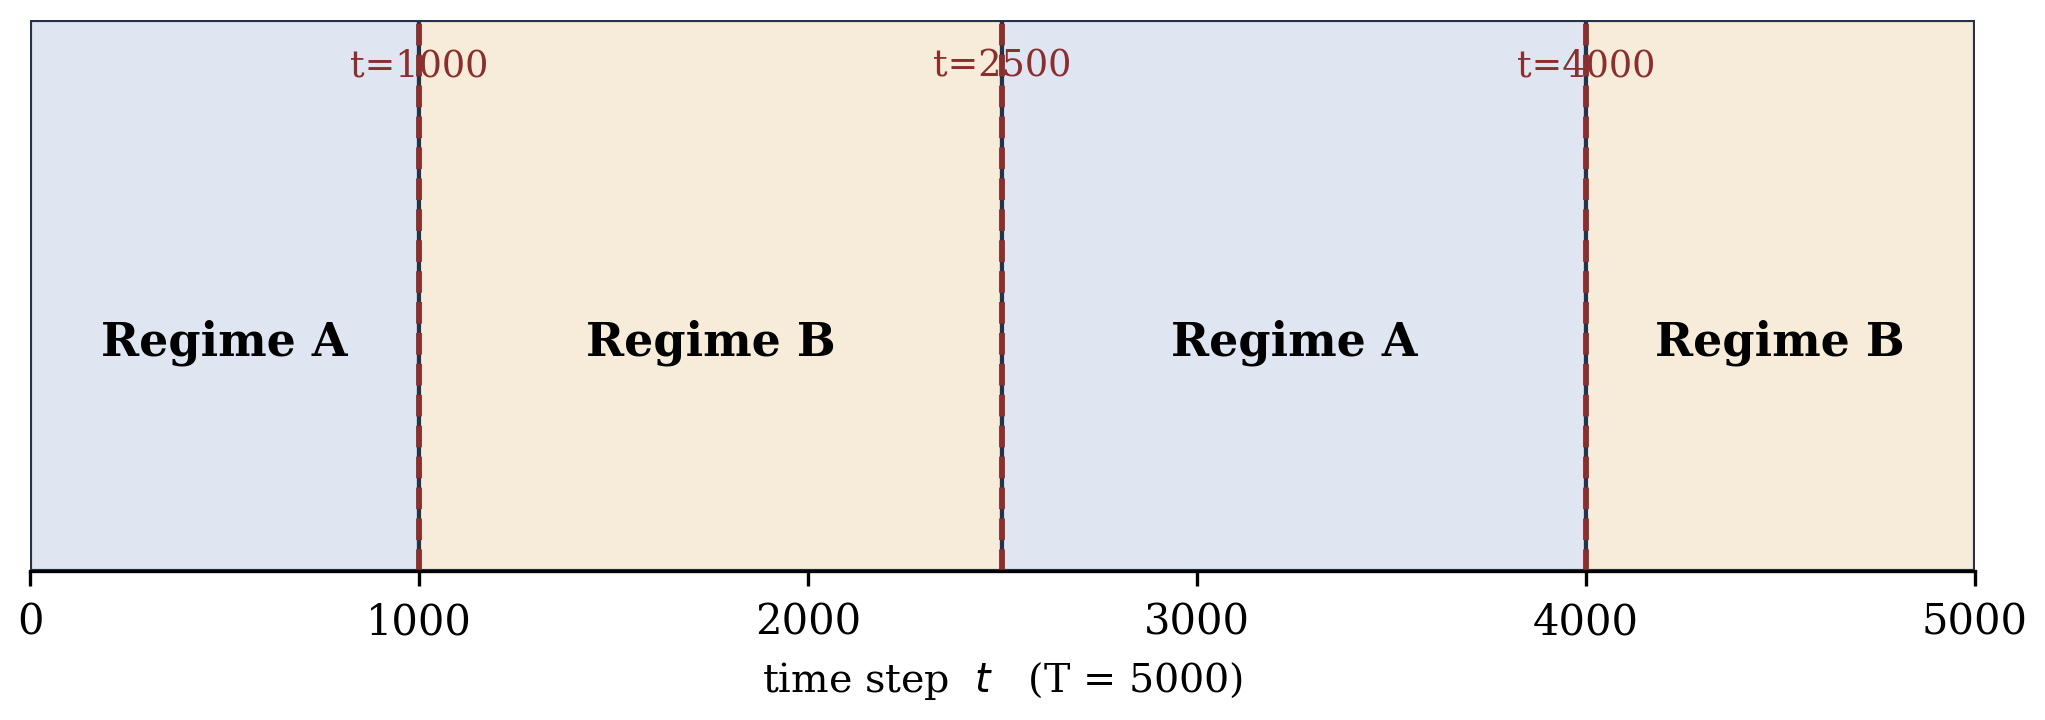
\includegraphics[width=\columnwidth]{figs/image3.png}
\caption{\textbf{Recurring-regime timeline used by the synthetic generator.} The return to Regime A at $t=2500$--$4000$ tests whether persistent memory accelerates recovery of a previously seen structure.}
\label{fig:timeline}
\end{figure}

\subsection{Baselines}
\label{sec:baselines}
The reported references include SCA, Rolling OLS, and CD-NOD. In the completed d=50, L=4 held-out stress test, Rolling OLS uses a 250-observation window and updates every 10 observations. It has no change detector or graph-memory state. CD-NOD is evaluated only on the pre-specified canonical dynamic cell using Fisher-Z conditional-independence tests and a chronological domain index. A full CD-NOD sweep was not attempted. PCMCI+ is used only for the illustrative external series; no quantitative comparison with RPCMCI, CASTOR, or FANTOM is reported.

\subsection{Evaluation Metrics}
\label{sec:metrics}
Edges are declared present by a fixed absolute coefficient threshold. We report precision, recall, F1, and structural Hamming distance (SHD). Stable-edge recall is the fraction of stable true edges remaining above the decision threshold over the post-change horizon. Per-edge recovery delay is reported for changed edges. Whole-graph recovery delay requires the entire predicted graph to equal the truth and is therefore a censored secondary diagnostic, not a primary endpoint. Change-detection rate records whether a detector fires in a post-change horizon; false-alarm rate records firing on stationary opportunities.

\subsection{Statistical Testing}
\label{sec:stats}
Paired comparisons between SCA and Rolling OLS are conducted with two-sided paired sign-flip randomisation tests (100,000 draws), reported alongside paired bootstrap 95\% confidence intervals for the mean difference and paired Cohen's $d_z$ effect sizes. All reported comparisons across metrics are Holm-corrected for multiple testing \cite{r15}. SCA is compared against CD-NOD only on the pre-specified canonical dynamic cell, without a paired statistical test across a factorial sweep, since CD-NOD was not run on the full design.

\subsection{Hyperparameter Selection}
\label{sec:hyper}
For the completed d=50, L=4 stress test, a fractional-factorial joint screen on tuning seeds 0--19 selected a dimension-aware local window, ridge alpha, persistence decay, and deviation scale. The detector threshold was calibrated from stationary null scores to target an eligible-update false-alarm rate of 0.05. The frozen configuration is $W=1000$, $D=500$, ridge alpha $=1.0$, persistence decay $=0.97$, deviation scale $=0.10$, and detector threshold $=0.3314109445$. The fixed edge-decision threshold remains 0.15. Earlier one-factor sensitivity results are retained as diagnostics only, not as the selection procedure.

\subsection{External Benchmark}
\label{sec:external}
In addition to the factorial design, SCA and PCMCI+ are tested on the \texttt{wt\_\allowbreak walks\_\allowbreak v1} / \texttt{actuators\_\allowbreak random\_\allowbreak walk\_\allowbreak 2} series from the Causal Chambers wind-tunnel testbed \cite{r12}. This series has 32 variables that are aligned with a graph structure and contains 10,000 observations arranged in order. The lags from 1 to 10 are combined into a single lag-agnostic task for directed-edge recovery. This is not a benchmark suite but a single physical data series. The results, found in Section~\ref{res:chambers}, are presented as an illustrative validation rather than as proof of reliability across real-world situations.

\begin{figure}[!t]
\centering
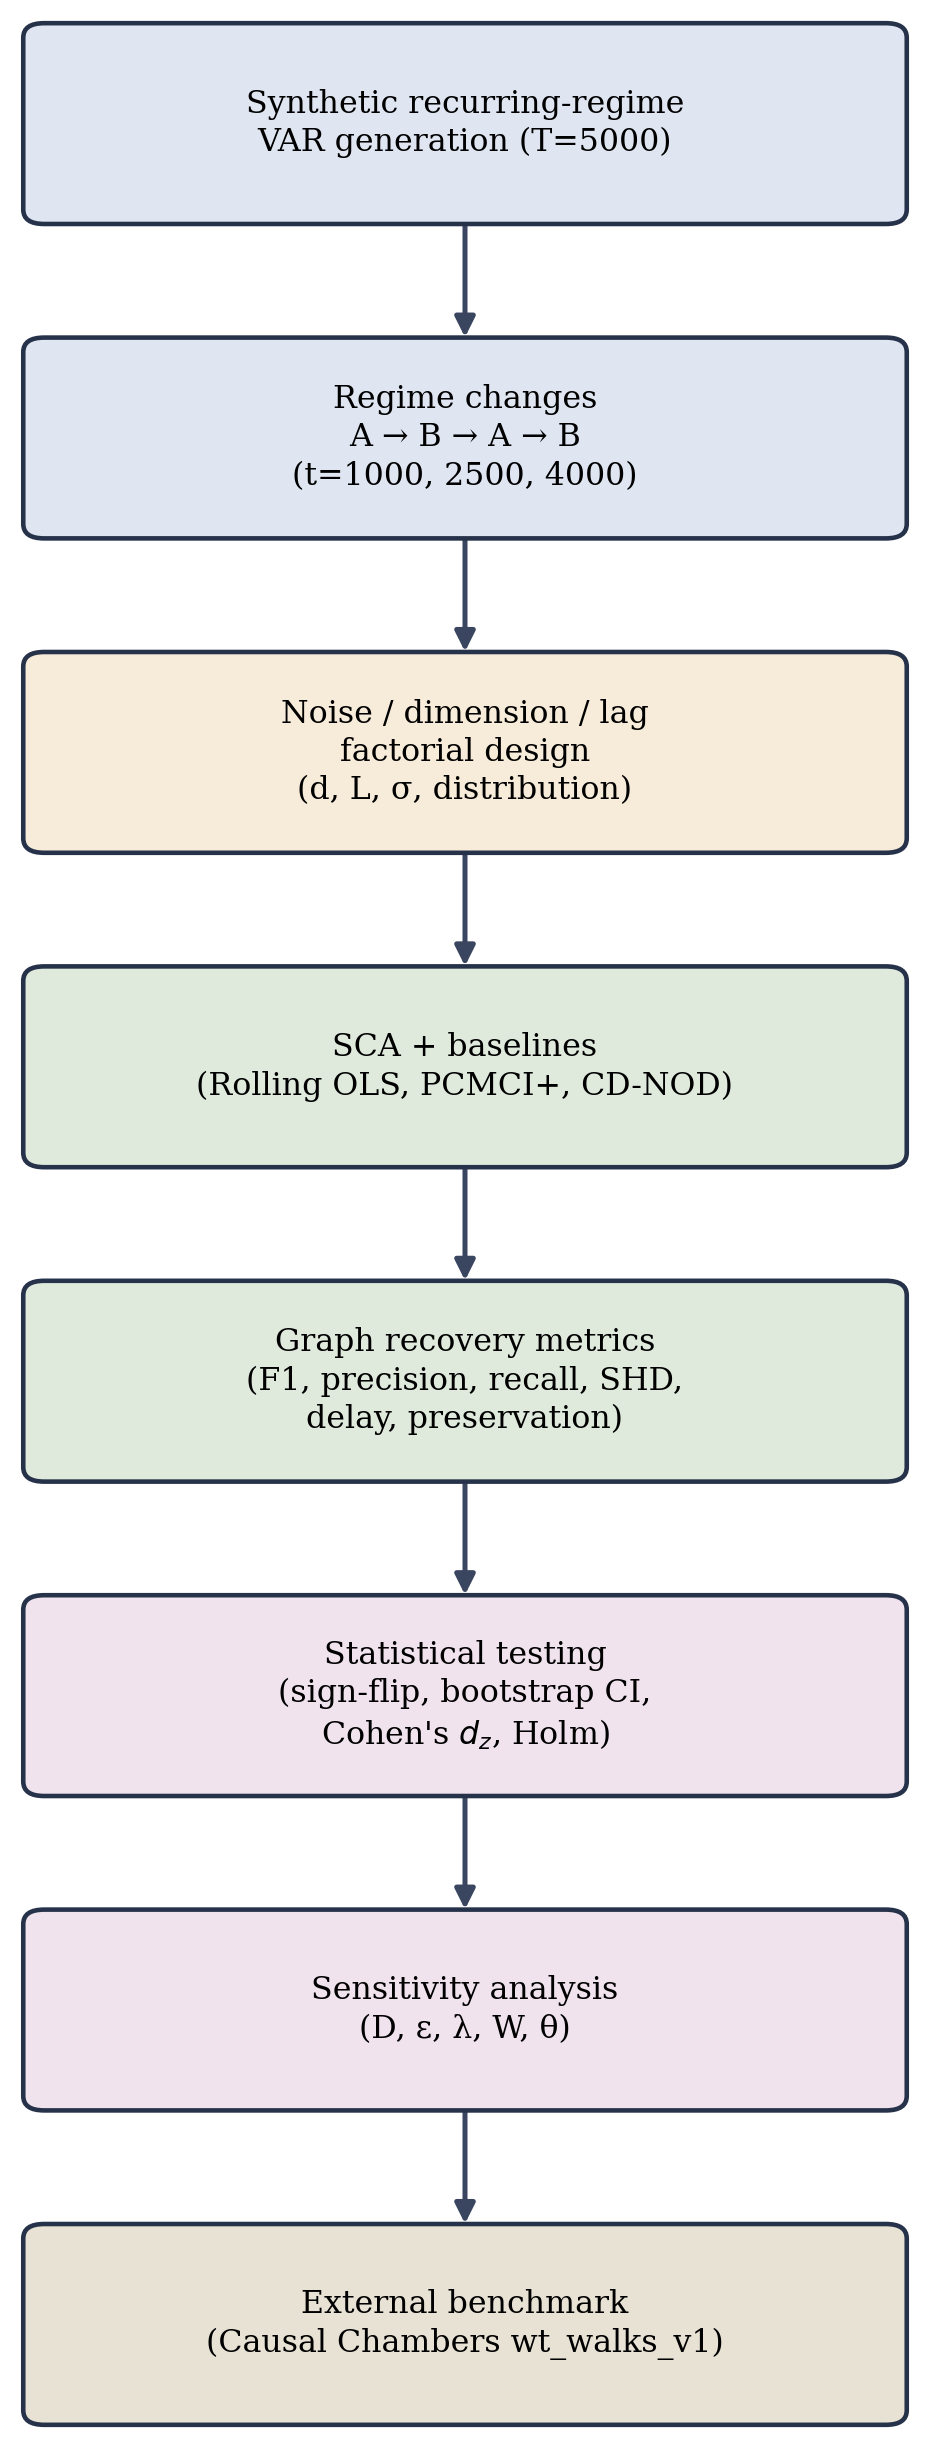
\includegraphics[width=0.68\columnwidth]{figs/image4.png}
\caption{\textbf{Experimental pipeline} from synthetic-data generation through the external benchmark.}
\label{fig:pipeline}
\end{figure}

%=====================================================================
\section{Results}
\label{sec:results}

\subsection{Canonical Dynamic Comparison}
\label{res:canonical}
Table~\ref{tab:canonical} presents the results for the pre-specified canonical dynamic cell ($d=4$, $L=2$, Gaussian noise, $\sigma=0.10$) comparing three methods: SCA, Rolling OLS and CD-NOD. SCA achieves higher precision than both baseline methods and shows a shorter adaptation delay compared to CD-NOD. However, CD-NOD reaches the highest F1 score among the three at 0.775, while SCA scores 0.637 and Rolling OLS scores 0.617. This better F1 performance comes from CD-NOD's higher recall (1.000 versus 0.551 for SCA). In addition, CD-NOD delivers perfect stable-edge preservation and flawless change detection in this cell. SCA, on the other hand, has a detection rate of $1.000\pm0.000$ with a false-alarm rate of $0.091\pm0.001$. We state these findings directly rather than framing precision or delay as an overall win. On this canonical condition, CD-NOD's regime-aware summary-graph approach recovers more of the true edge set than SCA does, at the cost of following the graph less conservatively.

\begin{table*}[!t]
\caption{Legacy fixed-configuration diagnostic: SCA vs.\ Rolling OLS vs.\ CD-NOD ($d=4$, $L=2$, Gaussian, $\sigma=0.10$; mean$\pm$s.d.). This table is not primary evidence for the jointly tuned protocol.}
\label{tab:canonical}
\centering
\small
\setlength{\tabcolsep}{6pt}
\begin{tabular}{lcccccc}
\toprule
\textbf{Method} & \textbf{Prec.} & \textbf{Recall} & \textbf{F1} & \textbf{SHD} & \textbf{Delay} & \textbf{Stable}\\
\midrule
SCA         & $0.869\pm0.042$ & $0.551\pm0.081$ & $0.637\pm0.065$ & $2.508\pm0.270$ & $456.3\pm51.5$ & $0.626\pm0.116$\\
Rolling OLS & $0.806\pm0.037$ & $0.537\pm0.042$ & $0.617\pm0.034$ & $2.352\pm0.154$ & $386.5\pm81.9$ & $0.582\pm0.097$\\
CD-NOD      & $0.638\pm0.093$ & $1.000\pm0.000$ & $0.775\pm0.069$ & $2.400\pm0.940$ & $500.0\pm0.0$  & $1.000\pm0.000$\\
\bottomrule
\end{tabular}
\end{table*}

CD-NOD's adaptation delay of 500.0 (the length of the post-change evaluation window) indicates that its change-point procedure did not resolve a discrete adaptation time within the evaluated horizon for this cell, which should temper direct comparison of the delay column.

\subsection{Pooled Factorial Results}
\label{res:pooled}
Table~\ref{tab:factorial} shows representative cells drawn from the full factorial design (held-out seeds, mean$\pm$s.d.\ where available), and Table~\ref{tab:pooled} reports the paired statistical comparison between SCA and Rolling OLS pooled across all factorial conditions and held-out seeds.

\begin{table}[!t]
\caption{Legacy fixed-configuration diagnostic (held-out seeds). This table is not primary evidence for the jointly tuned protocol.}
\label{tab:factorial}
\centering
\footnotesize
\setlength{\tabcolsep}{3pt}
\begin{tabular}{llccccc}
\toprule
\textbf{Condition} & \textbf{Method} & \textbf{Prec.} & \textbf{Rec.} & \textbf{F1} & \textbf{SHD} & \textbf{Delay}\\
\midrule
$d{=}4,L{=}1,\sigma{=}0.05$ & Rolling & 0.934 & 0.891 & 0.906 & 0.640 & 173.7\\
$d{=}4,L{=}1,\sigma{=}0.05$ & SCA     & 0.917 & 0.908 & 0.908 & 0.697 & 305.3\\
\addlinespace[2pt]
$d{=}4,L{=}1,\sigma{=}0.10$ & Rolling & 0.873 & 0.526 & 0.631 & 2.090 & 401.8\\
$d{=}4,L{=}1,\sigma{=}0.10$ & SCA     & 0.878 & 0.522 & 0.626 & 2.152 & 483.3\\
\addlinespace[2pt]
$d{=}4,L{=}1,\sigma{=}0.25$ & Rolling & 0.165 & 0.049 & 0.074 & 3.975 & 500.0\\
$d{=}4,L{=}1,\sigma{=}0.25$ & SCA     & 0.041 & 0.029 & 0.028 & 4.075 & 500.0\\
\addlinespace[2pt]
$d{=}50,L{=}1,\sigma{=}0.05$ & SCA    & 0.737 & 0.921 & 0.817 & 20.358 & ---\\
$d{=}50,L{=}2,\sigma{=}0.05$ & SCA    & 0.246 & 0.883 & 0.384 & 142.407 & ---\\
$d{=}50,L{=}4,\sigma{=}0.05$ & SCA    & 0.067 & 0.751 & 0.121 & 509.517 & ---\\
\bottomrule
\end{tabular}
\end{table}

Stable-edge preservation for these same cells (not shown in Table~\ref{tab:factorial} for space) is 0.939/0.993 (Rolling/SCA) at $d=4$, $\sigma=0.05$; 0.575/0.587 at $d=4$, $\sigma=0.10$; 0.067/0.011 at $d=4$, $\sigma=0.25$; and 0.968, 0.928, 0.847 for SCA at $d=50$ with $L=1,2,4$ respectively.

Two trends emerge in Table~\ref{tab:factorial}: first, as dimension and noise drop to low values ($d=4$, $\sigma=0.05$), SCA and Rolling OLS achieve similar F1, though SCA exhibits a considerably longer adaptation delay (305.3 vs.\ 173.7 steps), due to the conservative bias of the persistence gate: SCA waits for a substantial signal before declaring a change, whereas Rolling OLS always reacts to a new data window; second, with increasing dimension ($d=50$), there is a severe drop in F1 score as the lag order $L$ rises from 1 to 4 ($0.817\to0.384\to0.121$), mostly attributable to a large decrease in precision ($0.737\to0.246\to0.067$), while recall remains relatively high; correspondingly, SHD increases by more than an order of magnitude ($20.4\to142.4\to509.5$), reflecting the higher number of candidate edges at large $d$ and $L$. Section~\ref{res:failure} demonstrates that the $L=4$ cell also corresponds to a failure in change detection.

\begin{figure}[!t]
\centering
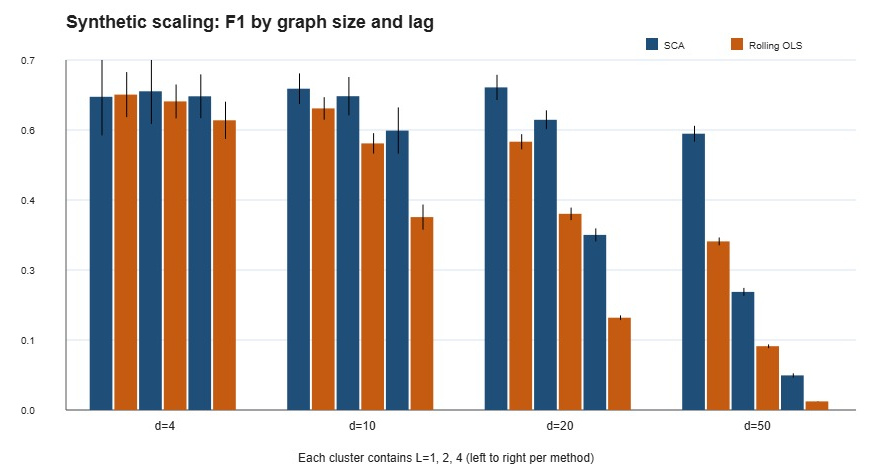
\includegraphics[width=\columnwidth]{figs/image5.png}
\caption{\textbf{Synthetic scaling:} mean F1 by graph dimension ($d$) and lag order ($L=1,2,4$ within each cluster) for SCA vs.\ Rolling OLS, illustrating the F1 collapse at high $d$ and $L$ described in Section~\ref{res:pooled}.}
\label{fig:scaling}
\end{figure}

\begin{table}[!t]
\caption{Legacy fixed-configuration diagnostic: pooled SCA vs.\ Rolling OLS comparison. These statistics are not used for primary claims.}
\label{tab:pooled}
\centering
\footnotesize
\setlength{\tabcolsep}{4.5pt}
\begin{tabular}{lcccc}
\toprule
\textbf{Metric} & $\boldsymbol{\Delta}$ & \textbf{95\% CI} & $\boldsymbol{d_z}$ & \textbf{Holm} $\boldsymbol{p}$\\
\midrule
Precision & $+0.0774$ & $[0.0762,\,0.0787]$ & $26.21$ & 0.00012\\
Recall    & $-0.0206$ & $[-0.0212,\,-0.0199]$ & $-14.20$ & 0.00012\\
F1        & $+0.0498$ & $[0.0492,\,0.0505]$ & $34.77$ & 0.00012\\
SHD       & $-244.20$ & $[-244.44,\,-243.95]$ & $-419.36$ & 0.00015\\
Delay     & $+0.575$  & $[-0.507,\,1.757]$ & $0.22$ & 0.71227\\
Stable    & $-0.0106$ & $[-0.0119,\,-0.0091]$ & $-3.19$ & 0.00012\\
\bottomrule
\end{tabular}
\end{table}

Pooled across the full factorial design, SCA shows a statistically significant improvement over Rolling OLS in precision, F1, and SHD (all Holm $p<0.001$), at the cost of a small but significant reduction in recall and in stable-edge preservation (both Holm $p<0.001$). The pooled SHD difference of $-244.20$ is large in absolute terms, but this magnitude is driven substantially by the high-$d$, high-$L$ cells in which SHD scales with the number of candidate edges ($d^2(L+1)$); it should not be read as a uniform per-cell improvement of that size. The aggregate adaptation-delay difference ($+0.575$ steps) is not statistically distinguishable from zero (Holm $p=0.712$, $d_z=0.22$): averaged across the whole factorial design, SCA is neither reliably faster nor reliably slower than Rolling OLS at fully recovering a post-change edge set, even though the two methods diverge substantially in individual cells (Table~\ref{tab:factorial}).

\subsection{Sensitivity Analysis}
\label{res:sens}
Table~\ref{tab:sens} reports a one-factor-at-a-time sensitivity sweep over SCA's five principal hyperparameters, performed on the tuning seeds (0--19) and held fixed at their selected value elsewhere in the row.

\begin{table}[!t]
\caption{Sensitivity Analysis (tuning seeds; one factor varied at a time)}
\label{tab:sens}
\centering
\footnotesize
\setlength{\tabcolsep}{5pt}
\begin{tabular}{llccc}
\toprule
\textbf{Parameter} & \textbf{Value} & \textbf{F1} & \textbf{SHD} & \textbf{FAR}\\
\midrule
$D$ (window)      & 50    & 0.537 & 3.604 & ---\\
$D$ (window)      & 100   & 0.531 & 3.854 & ---\\
$D$ (window)      & 200   & 0.523 & 4.363 & ---\\
\addlinespace[2pt]
$\epsilon$ (tolerance) & 0.025 & 0.506 & 4.261 & ---\\
$\epsilon$ (tolerance) & 0.05  & 0.531 & 3.854 & ---\\
$\epsilon$ (tolerance) & 0.10  & 0.575 & 3.225 & ---\\
\addlinespace[2pt]
$\lambda$ (decay) & 0.70  & 0.517 & 4.077 & ---\\
$\lambda$ (decay) & 0.90  & 0.531 & 3.854 & ---\\
$\lambda$ (decay) & 0.97  & 0.540 & 3.762 & ---\\
\addlinespace[2pt]
$W$ (local win.)  & 50    & 0.408 & 6.051 & ---\\
$W$ (local win.)  & 100   & 0.531 & 3.854 & ---\\
$W$ (local win.)  & 200   & 0.609 & 2.824 & ---\\
\addlinespace[2pt]
$\theta$ (threshold) & 0.20 & 0.531 & 3.858 & 0.089\\
$\theta$ (threshold) & 0.25 & 0.547 & 3.734 & 0.057\\
$\theta$ (threshold) & 0.30 & 0.567 & 3.608 & 0.017\\
\bottomrule
\end{tabular}
\end{table}

The one-factor results are descriptive diagnostics for the legacy configuration. They do not estimate parameter interactions and were not used to select the completed stress-test configuration; joint, dimension-aware selection and null calibration were used instead.

\begin{figure}[!t]
\centering
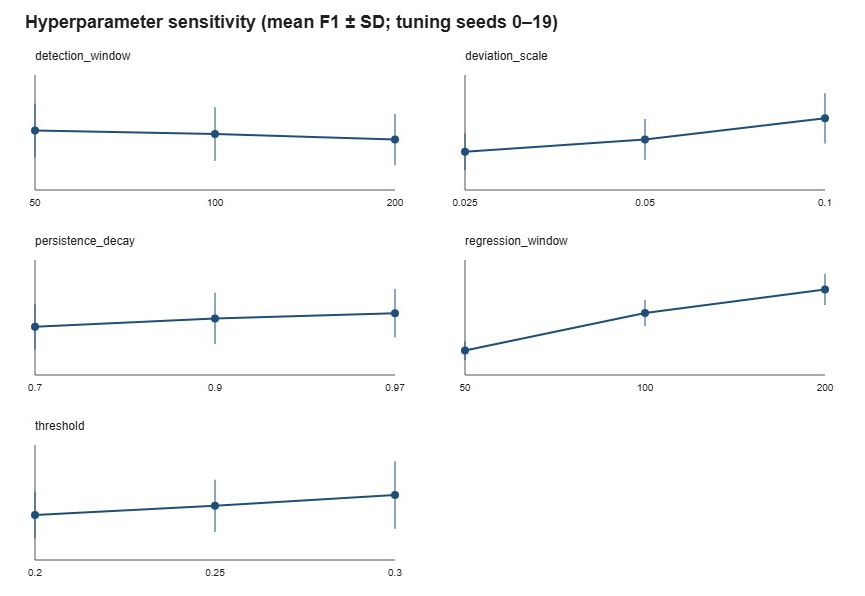
\includegraphics[width=\columnwidth]{figs/image6.png}
\caption{\textbf{Hyperparameter sensitivity:} mean F1 $\pm$ SD across tuning seeds (0--19) for each of SCA's five principal hyperparameters (Section~\ref{res:sens}).}
\label{fig:sens}
\end{figure}

\subsection{Ablation Study}
\label{res:ablation}
The development benchmark (\texttt{regime\_\allowbreak change\_\allowbreak a1.csv}: $T=5000$, $d=4$, $L=2$, Gaussian noise scale 0.1, seed 42, single change at $t=2500$) is a smaller, earlier diagnostic instance where three lagged/stable relationships are unchanged across the transition, one contemporaneous edge is removed, and one lagged edge is added. Since the estimator is past-only and cannot recover contemporaneous directions, this benchmark is treated as a diagnostic smoke test instead of primary manuscript evidence, and Table~\ref{tab:ablation} reports the before/after metrics for the full SCA model and two ablations.

\begin{table*}[!t]
\caption{Development Benchmark / Ablation (\texttt{regime\_\allowbreak change\_\allowbreak a1.csv})}
\label{tab:ablation}
\centering
\small
\setlength{\tabcolsep}{6pt}
\begin{tabular}{lccccccc}
\toprule
\textbf{Method} & \textbf{F1 pre} & \textbf{F1 post} & \textbf{SHD pre} & \textbf{SHD post} & \textbf{Stable} & \textbf{Detect.} & \textbf{Delay}\\
\midrule
Full SCA        & 0.5714 & 0.7273 & 6 & 3   & 0.9591 & 0.8712 & 80\\
No Persist.     & 0.4615 & 0.6667 & 7 & 4   & 0.9347 & 0.7780 & 41\\
Global Only     & 0.4286 & 0.5333 & 8 & 7   & 0.9187 & 0.7580 & 27\\
Rolling regr.   & 1.0000 & 0.7500 & 0 & 2   & 0.7603 & 0.8592 & 352\\
PCMCI+ (static) & 0.8889 & N/A    & 1 & N/A & ---    & ---    & ---\\
\bottomrule
\end{tabular}
\end{table*}

The development ablation is a single diagnostic instance. Its qualitative ordering is compatible with the intended roles of persistence and edgewise gating, but it is not a multi-seed estimate of a general selectivity advantage. The ``Stable'' column is stable-edge recall; its whole-graph delay column is a censored secondary diagnostic.

\begin{figure}[!t]
\centering
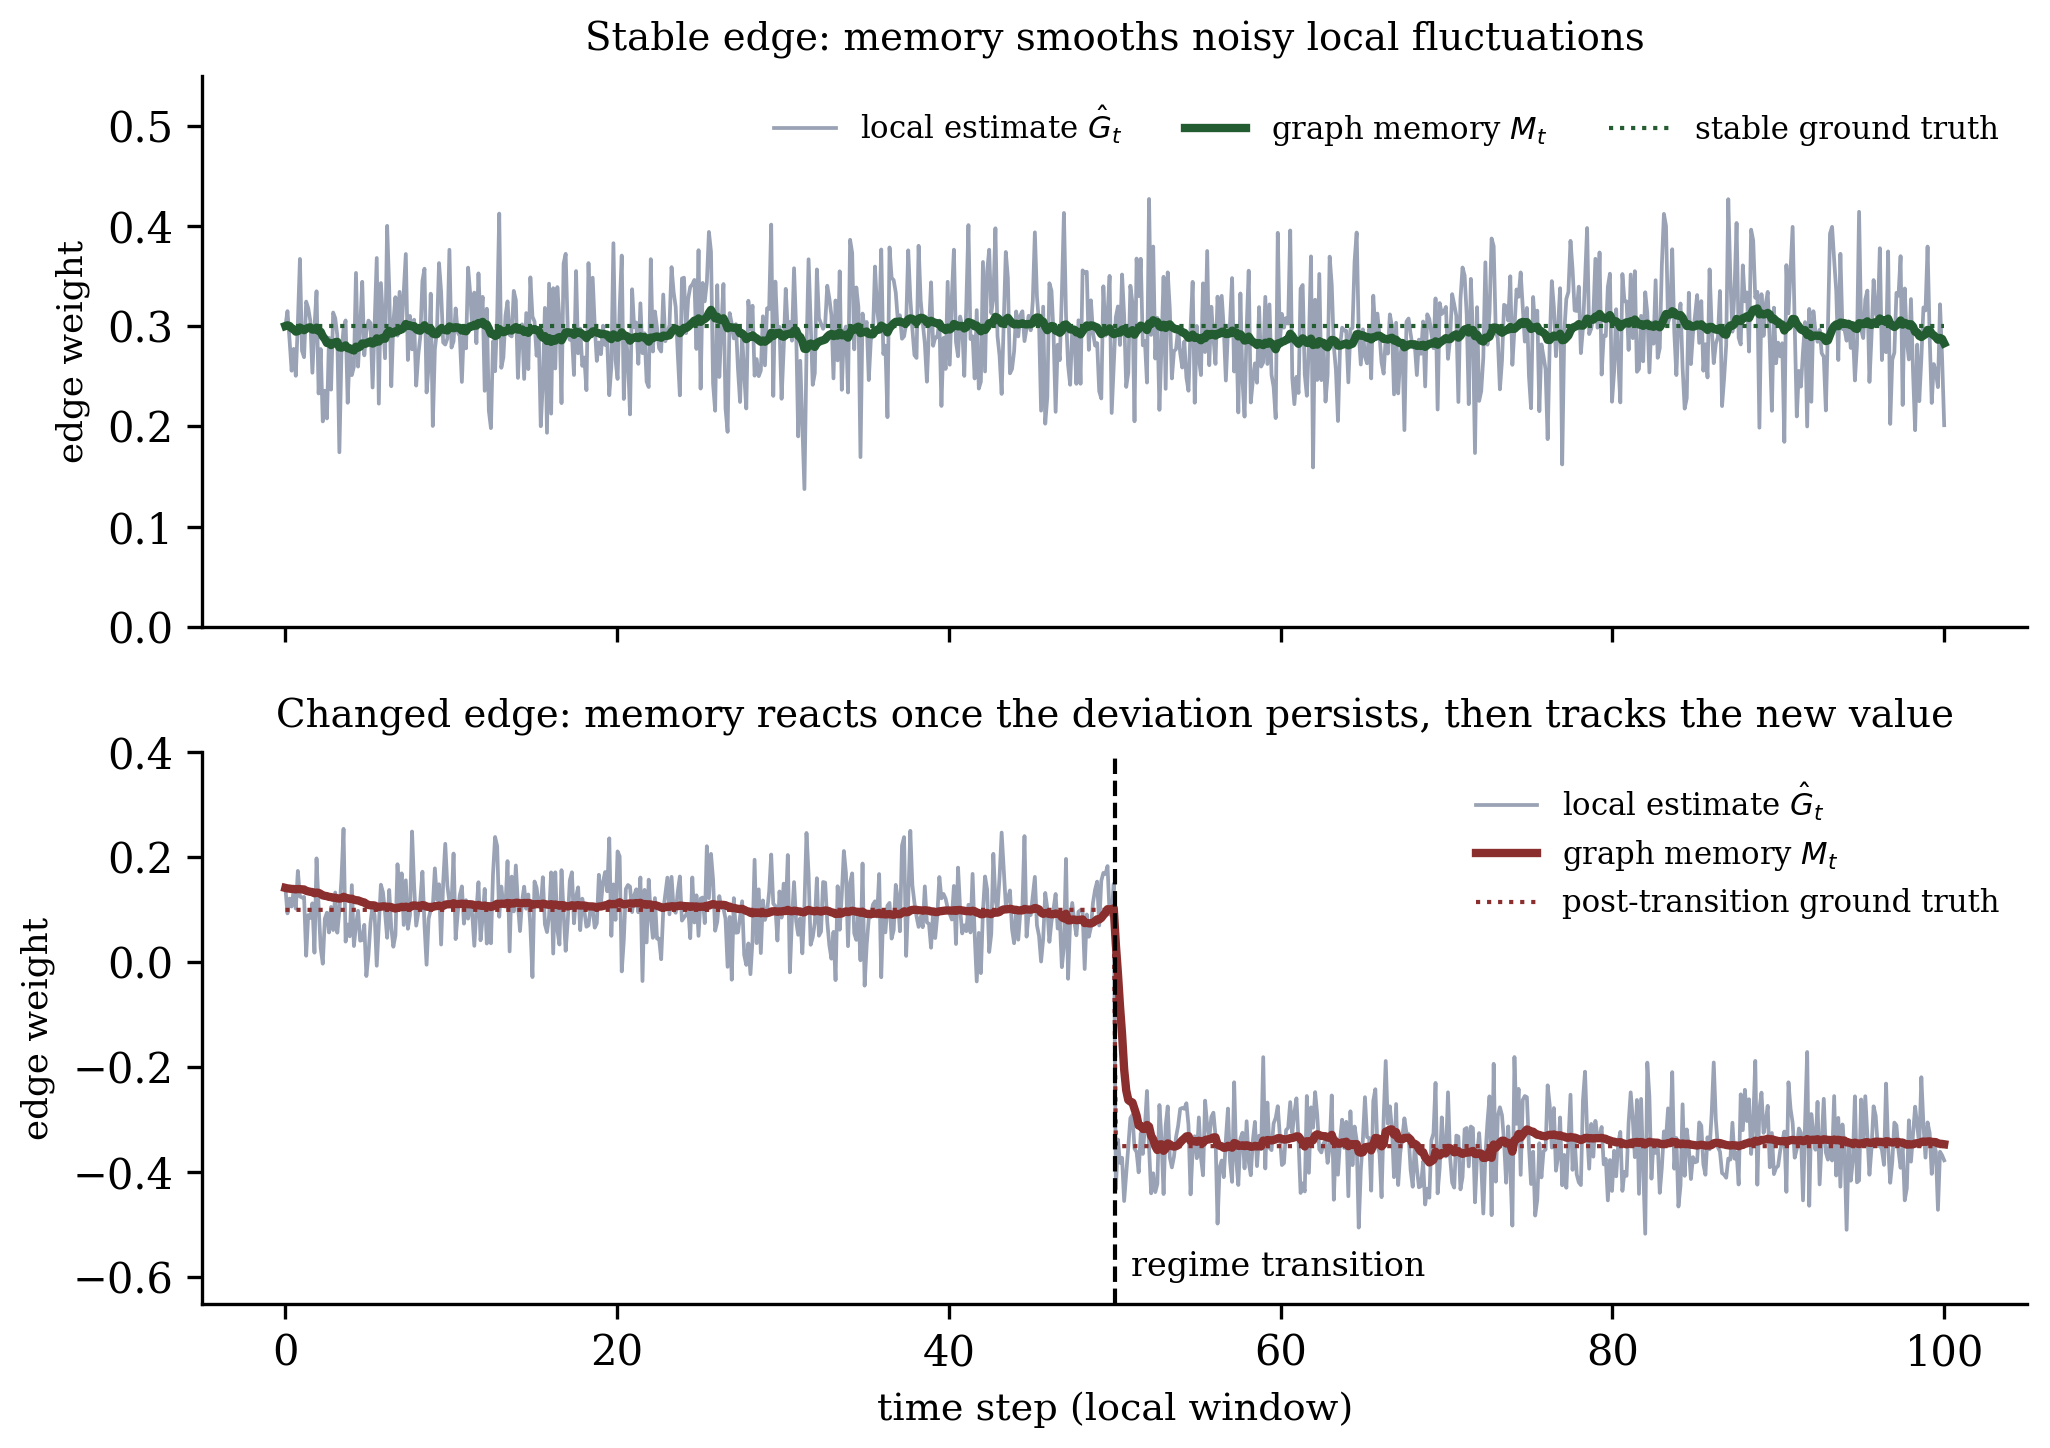
\includegraphics[width=\columnwidth]{figs/image7.png}
\caption{\textbf{Conceptual edge trajectory: local estimate vs.\ graph memory.} Memory smooths a stable edge's noisy local fluctuations (top) but, once a deviation is detected and persists, tracks a changed edge to its new value (bottom).}
\label{fig:trajectory}
\end{figure}

\subsection{Plasticity Analysis}
\label{res:plast}
Table~\ref{tab:plast} reports the average realised plasticity rate on changed edges versus stable edges for the full model and the two ablations from Section~\ref{res:ablation}.

\begin{table}[!t]
\caption{Plasticity Analysis: Changed- vs.\ Stable-Edge Update Rates}
\label{tab:plast}
\centering
\footnotesize
\setlength{\tabcolsep}{6pt}
\begin{tabular}{lccc}
\toprule
\textbf{Method} & \textbf{Changed} & \textbf{Stable} & \textbf{Ratio}\\
\midrule
Full SCA       & 0.0231 & 0.0204 & $1.132\times$\\
No Persistence & 0.0349 & 0.0307 & $1.137\times$\\
Global Only    & 0.1400 & 0.1400 & $1.000\times$\\
\bottomrule
\end{tabular}
\end{table}

The Global-Only ablation applies the same rate to changed and stable edges by construction (ratio $1.000\times$), confirming that it has no edge-level selectivity. Adding persistence decreases both the changed- and stable-edge rates substantially compared to No Persistence ($0.0349\to0.0231$ and $0.0307\to0.0204$, respectively), but only slightly changes the ratio between them ($1.137\times\to1.132\times$). This is a genuinely nuanced finding: persistence's main empirical effect on this benchmark is to scale down plasticity overall---to act as a conservative brake on both changed and stable edges alike---rather than to sharply raise the amount by which changed edges are treated differently than stable ones. Edge-level selectivity (comparing Global Only to No Persistence) is what causes most of the ratio's departure from $1.0\times$ in the first place.

\subsection{External Benchmark}
\label{res:chambers}
Table~\ref{tab:chambers} reports results on the \texttt{wt\_\allowbreak walks\_\allowbreak v1} / \texttt{actuators\_\allowbreak random\_\allowbreak walk\_\allowbreak 2} Causal Chambers series (32 variables, 10,000 observations, lags 1--10 collapsed to lag-agnostic directed-edge recovery).

\begin{table}[!t]
\caption{Causal Chambers External Benchmark (\texttt{actuators\_\allowbreak random\_\allowbreak walk\_\allowbreak 2})}
\label{tab:chambers}
\centering
\footnotesize
\setlength{\tabcolsep}{3pt}
\begin{tabular}{llccccc}
\toprule
\textbf{Method} & \textbf{TP/FP/FN} & \textbf{Prec.} & \textbf{Rec.} & \textbf{F1} & \textbf{SHD} & \textbf{Time (s)}\\
\midrule
SCA    & 24/125/18 & 0.161 & 0.571 & 0.251 & 143 & 56.0\\
PCMCI+ & 1/33/41   & 0.029 & 0.024 & 0.026 & 74  & 87.1\\
\bottomrule
\end{tabular}
\end{table}

SCA achieves a much higher F1 score than PCMCI+ on this dataset (0.251 compared to 0.026), mainly due to its higher recall value; however, PCMCI+'s SHD is also lower (74 versus 143) because its predictions are much sparser than SCA's. In fact, fewer predicted edges result in fewer false positives, but such an inference implies that most of the true edges are missed by PCMCI+. We do not interpret PCMCI+'s lower SHD as a sign of being a better algorithm in this case, nor do we make generalisations based on a single data set that may not justify any type of conclusion about real-life efficacy of any of these methods.

\subsection{High-Dimensional Stress-Test Repair}
\label{res:failure}
The legacy small-window OLS configuration is ill conditioned at $d=50$, $L=4$: it has approximately 200 lagged predictors per equation but only about 196 local observations. The completed repair uses dimension-aware windows and ridge regularisation. On the held-out Gaussian $\sigma=0.10$ d=50, L=4 cell, the frozen configuration ($W=1000$, $D=500$, ridge alpha $=1.0$, detector threshold $=0.3314109445$) obtains F1 $0.576\pm0.036$ and AUPRC $0.831\pm0.014$ over seeds 20--39. Its matched stationary-null eligible-update false-alarm rate is $0.044\pm0.014$. This targeted repair does not validate the method over the full factorial design.

\begin{figure}[!t]
\centering
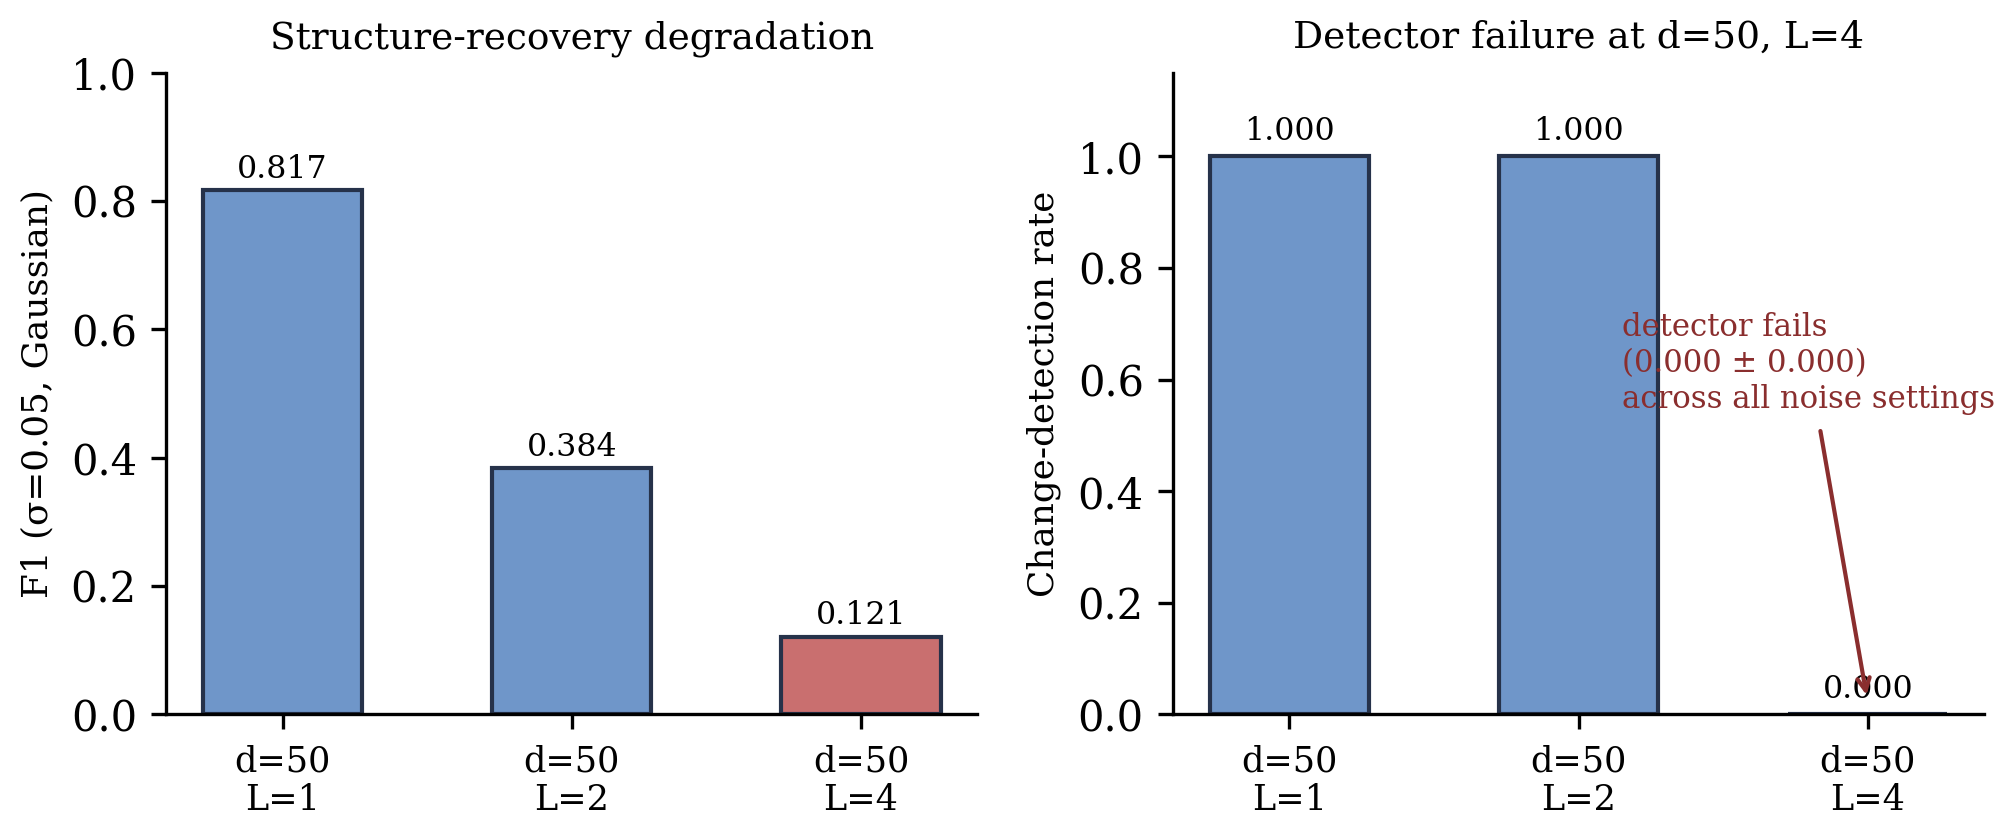
\includegraphics[width=\columnwidth]{figs/image8.png}
\caption{\textbf{Legacy fixed-configuration diagnostic.} This figure illustrates the small-window high-dimensional degradation that motivated the jointly tuned d=50, L=4 repair; it is not a result for the repaired configuration.}
\label{fig:failure}
\end{figure}

%=====================================================================
\section{Discussion}
\label{sec:discussion}
Selective, edge-level adaptation using memory and persistence is the contribution of SCA. Rather than claiming overall superiority over all competing methods, the data presented here demonstrate that (i) SCA improves precision and F1 over Rolling OLS with only a minor loss in recall, as shown in Table~\ref{tab:pooled}; (ii) somewhat disappointingly, SCA offers no improvement over Rolling OLS in stable-edge preservation, actually showing an average difference of $-0.0106$ (Holm $p=0.00012$), which suggests that the memory mechanism used by SCA is not better, in terms of stable-edge preservation, than simple re-estimation at every step, despite the demonstrable benefit over Rolling OLS on the small development benchmark of Table~\ref{tab:ablation}; and (iii) in the comparison of overall adaptation delay, SCA and Rolling OLS are approximately on the same level, with neither method significantly better than the other across the factorial design ($p=0.71227$): throughout the factorial design, neither algorithm was reliably faster in its ability to fully adapt to a new edge set following a change point, despite noticeable differences in delay in individual cells and in the development benchmark.

In the canonical dynamic scenario, the F1 performance of CD-NOD exceeds that of SCA (0.775 vs.\ 0.637) because CD-NOD has perfect recall in that cell. Meanwhile, SCA trades lower recall for higher precision and a shorter adaptation delay than CD-NOD. Rolling OLS does very well in terms of the raw score of local-graph recovery. In particular, it performs perfectly before the occurrence of a change (see Table~\ref{tab:ablation}, F1$=$1.0000 for the development benchmark), which is not surprising because it uses only the most recent information and does not retain any historical information that contradicts it. SCA uses a different approach, which gives it better resistance to unnecessary changes (Table~\ref{tab:ablation}, unnecessary-change rate of 0.0409 as opposed to 0.2397 for Rolling OLS), but introduces inertia that leads to longer adaptation delays in some cells (see Table~\ref{tab:factorial}), even though in the aggregate comparison those delay differences are not significant.

High-dimensional, high-lag settings expose an important failure mode that must be discussed explicitly rather than implicitly: at $d=50$, $L=4$ the change detector's detection rate collapses to 0.000 across every evaluated noise condition (Section~\ref{res:failure}), coinciding with severe F1 and SHD degradation. This traces to the detector's fixed top-$k$ design, which becomes under-powered when the number of candidate edges ($d^2(L+1)$) grows large compared to the fixed number of slots examined. The external Causal Chambers benchmark (Section~\ref{res:chambers}) contains only one physical series, so its results should be read as an illustrative check rather than a validated real-world evaluation; and the current experiments do not fully test nonlinear generating mechanisms or heteroscedastic noise, both of which are addressed by generative frameworks such as FANTOM \cite{r8} but are outside the present study's scope. The one-factor-at-a-time sensitivity analysis (Section~\ref{res:sens}) characterises each hyperparameter's marginal effect, but not their interactions. Finally, unlike Rhino \cite{r4} or FANTOM \cite{r8}, the present work provides no theoretical convergence, bias, or identifiability proof for the persistence-gated memory filter; SCA's justification is empirical, and its use of a regression-based evidence score as a proxy for edge presence relies informally on established identifiability results for additive-noise causal models \cite{r8,r14} rather than on a dedicated proof of its own.

%=====================================================================
\section{Limitations and Future Work}
\label{sec:limits}

\subsection{Limitations}
We summarise the limitations discussed throughout the paper in one place. (1) SCA is a past-only, Granger-style estimator: the lag-zero plane is fixed to zero and makes no claim about contemporaneous structural causal identification. (2) The change detector fails outright in the high-dimensional, high-lag regime tested here ($d=50$, $L=4$), where its detection rate drops to zero. (3) The detector's fixed top-$k$ design does not scale its sensitivity to the number of candidate edges, which is the root cause of (2). (4) Nonlinear generating mechanisms are not evaluated; all synthetic data are generated by a linear VAR process. (5) Heteroscedastic noise, of the kind explicitly modelled by FANTOM \cite{r8}, is not evaluated. (6) The external validation rests on a single Causal Chambers physical series, too little data to make a general real-world reliability claim. (7) RPCMCI, CASTOR, and FANTOM are discussed as related methods but were not run end-to-end on this study's factorial design, so no quantitative comparison against them is reported here. (8) The sensitivity analysis varies one hyperparameter at a time and cannot characterise interactions between parameters such as $D$, $\epsilon$, $\lambda$, $W$, and $\theta$. (9) No theoretical convergence, bias, or identifiability guarantee is provided for the persistence-gated memory filter.

\subsection{Future Work}
Several directions follow from the above limitations: (1) an adaptive or dimension-aware change detector, for example one that scales its score by the number of candidate edges or calibrates $k$ to $d$ and $L$ rather than using a fixed small constant; (2) direct factorial sweeps over selectivity and plasticity bounds ($[\amin,\amax]$) rather than the current one-factor-at-a-time protocol to expose interaction effects; (3) evaluation on nonlinear and heteroscedastic data generators, potentially by replacing the OLS-based local evidence score with a learned, history-dependent likelihood in the spirit of Rhino \cite{r4} or FANTOM's conditional normalising flows \cite{r8} at the cost of the current pipeline's training-free simplicity; (4) additional real-world benchmarks beyond the single Causal Chambers series used here, including EEG or other biomedical series with documented heteroscedastic noise \cite{r8,r13}; (5) a full quantitative comparison against RPCMCI, CASTOR, and FANTOM on a shared factorial design; (6) multi-factor hyperparameter analysis (e.g., a designed experiment or Bayesian optimisation over the joint hyperparameter space); (7) theoretical analysis of the convergence and bias properties of the persistence-gated exponential memory filter; and (8) regime-aware memory mechanisms that combine SCA's edge-level selectivity with an explicit, discrete notion of regime identity, potentially recovering some of CD-NOD's and FANTOM's recall advantage without discarding SCA's precision and conservatism.

%=====================================================================
\section{Conclusion}
\label{sec:conclusion}
This paper introduces Selective Causal Adaptation, a training-free streaming framework which shifts the unit of adaptation in dynamic causal discovery from the graph as a whole to the individual edge, gating a persistent causal-graph memory with a multiplicative, edge-level plasticity rate that combines the impact of global change intensity, local deviation, and edge-specific persistence. Under the evaluated conditions, while SCA consistently improves precision and pooled F1 compared to a memory-free Rolling-OLS baseline at the cost of recall, it does not demonstrate a universal advantage in either stable-edge preservation or adaptation delay once results are aggregated across the full factorial design; CD-NOD achieves a higher F1 than SCA on the canonical dynamic condition by virtue of a significantly better recall; and a high-dimensional, high-lag stress test reveals a change-detector failure mode on which we advise caution as an honestly reported limitation rather than an exceptional capability. Two ablation experiments confirm the contribution of both the persistence gate and edge-level selectivity to the observed performance, while a detailed plasticity analysis reveals that persistence manifests primarily as a conservative dampening of adaptation rate, rather than a dramatic increase in contrast between changed and stable edges. We posit SCA as a lightweight alternative in applications where non-stationarity is expected to manifest at the edge level and a training-free update regime is desirable, rather than a replacement for regime-aware generative models such as CASTOR or FANTOM in settings which benefit from their greater flexibility and theoretical guarantees.

\section*{Acknowledgment}
The authors thank their department for computing resources used in the factorial evaluation reported in this paper.

%=====================================================================
\begin{thebibliography}{00}

\bibitem{r1} J. Runge, ``Discovering contemporaneous and lagged causal relations in autocorrelated nonlinear time series datasets,'' in \emph{Proc. Conf. Uncertainty Artif. Intell. (UAI)}, PMLR, 2020, pp. 1388--1397.

\bibitem{r2} X. Zheng, B. Aragam, P. K. Ravikumar, and E. P. Xing, ``DAGs with NO TEARS: Continuous optimization for structure learning,'' in \emph{Proc. Adv. Neural Inf. Process. Syst. (NeurIPS)}, vol. 31, 2018.

\bibitem{r3} R. Pamfil, N. Sriwattanaworachai, S. Desai, P. Pilgerstorfer, K. Georgatzis, P. Beaumont, and B. Aragam, ``DYNOTEARS: Structure learning from time-series data,'' in \emph{Proc. Int. Conf. Artif. Intell. Statist. (AISTATS)}, PMLR, 2020.

\bibitem{r4} W. Gong, J. Jennings, C. Zhang, and N. Pawlowski, ``Rhino: Deep causal temporal relationship learning with history-dependent noise,'' in \emph{Proc. Int. Conf. Learn. Represent. (ICLR)}, 2023.

\bibitem{r5} B. Huang, K. Zhang, J. Zhang, J. Ramsey, R. Sanchez-Romero, C. Glymour, and B. Sch{\"o}lkopf, ``Causal discovery from heterogeneous/nonstationary data,'' \emph{J. Mach. Learn. Res.}, vol. 21, no. 89, pp. 1--53, 2020.

\bibitem{r6} E. Saggioro, J. de Wiljes, M. Kretschmer, and J. Runge, ``Reconstructing regime-dependent causal relationships from observational time series,'' \emph{Chaos: An Interdisciplinary Journal of Nonlinear Science}, vol. 30, no. 11, 2020.

\bibitem{r7} A. Rahmani and P. Frossard, ``Causal temporal regime structure learning,'' in \emph{Proc. 28th Int. Conf. Artif. Intell. Statist. (AISTATS)}, PMLR, vol. 258, 2025, pp. 4546--4554.

\bibitem{r8} A. Rahmani and P. Frossard, ``Flow based approach for dynamic temporal causal models with non-Gaussian or heteroscedastic noises,'' in \emph{Proc. Adv. Neural Inf. Process. Syst. (NeurIPS)}, vol. 38, 2025.

\bibitem{r9} S. Mameche, L. Cornanguer, U. Ninad, and J. Vreeken, ``SPACETIME: Causal discovery from non-stationary time series,'' in \emph{Proc. AAAI Conf. Artif. Intell.}, vol. 39, no. 18, 2025, pp. 19405--19413.

\bibitem{r10} D. Xu, C. Ruan, E. Korpeoglu, S. Kumar, and K. Achan, ``Inductive representation learning on temporal graphs,'' in \emph{Proc. Int. Conf. Learn. Represent. (ICLR)}, 2020.

\bibitem{r11} M. H. Ferdous, E. Hossain, and M. O. Gani, ``TimeGraph: Synthetic benchmark datasets for robust time-series causal discovery,'' in \emph{Proc. 31st ACM SIGKDD Conf. Knowl. Discovery Data Mining (KDD)}, 2025.

\bibitem{r12} J. L. Gamella, J. Peters, and P. B{\"u}hlmann, ``Causal chambers as a real-world physical testbed for AI methodology,'' \emph{Nature Mach. Intell.}, vol. 7, no. 1, pp. 107--118, 2025.

\bibitem{r13} H. M. Huizenga and P. C. Molenaar, ``Equivalent source estimation of scalp potential fields contaminated by heteroscedastic and correlated noise,'' \emph{Brain Topogr.}, vol. 8, pp. 13--33, 1995.

\bibitem{r14} J. Peters, J. M. Mooij, D. Janzing, and B. Sch{\"o}lkopf, ``Causal discovery with continuous additive noise models,'' \emph{J. Mach. Learn. Res.}, vol. 15, no. 1, pp. 2009--2053, 2014.

\bibitem{r15} S. Holm, ``A simple sequentially rejective multiple test procedure,'' \emph{Scand. J. Statist.}, vol. 6, no. 2, pp. 65--70, 1979.

\end{thebibliography}

%=====================================================================
\section*{Author Biographies}

\begin{IEEEbiographynophoto}{Suyesha Saha}
is currently pursuing the B.Tech.\ degree in Computer Science and Engineering at Vellore Institute of Technology, Chennai, India. Her research interests include causal discovery, time-series analysis, and streaming machine learning systems.
\end{IEEEbiographynophoto}

\begin{IEEEbiographynophoto}{Ippili Sai Sahasra}
is currently pursuing the B.Tech.\ degree in Computer Science and Engineering at Vellore Institute of Technology, Chennai, India. Her research interests include statistical machine learning and dynamic graph estimation.
\end{IEEEbiographynophoto}

\begin{IEEEbiographynophoto}{Ananya Arumbakkam}
is currently pursuing the B.Tech.\ degree in Computer Science and Engineering at Vellore Institute of Technology, Chennai, India. Her research interests include non-stationary time-series modelling and empirical evaluation methodology for machine learning systems.
\end{IEEEbiographynophoto}

\begin{IEEEbiographynophoto}{Suhasini S}
is a faculty member in the School of Electronics Engineering at Vellore Institute of Technology, Chennai, India. Her research interests include signal processing and applied statistical modelling for physical and biomedical systems.
\end{IEEEbiographynophoto}

\vfill

\EOD

\end{document}
